\documentclass{rureport}
\svnid{$Id: example-proposal-detailed.tex 145 2016-08-16 11:56:53Z foley $}
%% Reykjavik University Proposal Template (detailed)
%% Written by Joseph Timothy Foley <foley AT ru DOT IS>

%% Fixmes are reminders of things that still need to be done.
%% The default fixmes are:  \fxnote{} \fxwarning{} \fxerror{} \fxfatal{} (same as \fixme{})
% if you want personalized fixmes, then register the authors here
% notice that the first field is 2 letters, the second is 3.
\FXRegisterAuthor{jf}{jtf}{foley}
% this registers \jfnote{}, \jfwarning{}, \jferror{}, \jffatal{}

%% declare the paths(s) where you graphics files can be found
\graphicspath{{graphics/}{Graphics/}{./}}

\author{Amin Fallahi\formatemail{afallahi@syr.edu}}  % My name, for the titlepage
\title{JavaScript Code Deobfuscation using Neural Program Learning Models}  % The title, for the titlepage
\course{Neural Program Learning Course Project Proposal}

\usepackage{hyperref} % must be last package loaded!
% it makes hyper-references (citations, URLs, etc) clickable
\begin{document} % this tells the compiler that it is time to make
                 % text to print instead of just getting ready.
\maketitle  % make a title page from the Title, Date, and Author
\listoffixmes{}


\section{Introduction}
One of the trending methods for improving software security and hiding program codes from users is JavaScript code obfuscation. JavaScript codes are meant to run on the browsers and are widely used to create dynamic content in most web-pages. Many content providers try to hide the code from the user to improve their security and obscure the real function of code. Using a simple obfuscation technique, the providers make their program secure against attackers and are able to inject malicious code that can help advertisement, tracking the user, collecting user info, cross-site scripting attack, etc. Obfuscation targets changing the code in a way that makes it hard for the human to understand what the code is actually doing by methods like changing variable/function names, altering execution order, loop unrolling, character encoding, etc.\\
In contrast, code deobfuscation methods try to gain as much information from obfuscated codes and extract the program from the unreadble code.\\
In this project, we use neural program learning methods to recover identifier (variables and functions) names from obfuscated JavaScript code. We study current JavaScript obfuscation and deobfuscation methods and how much identifier names the current approaches to deobfuscation can predict. Then, we implement a program learning model and train it using available data sets. Finally, we evaluate our work and try to optimize the model to achieve better performance than previous research. 

\section{Related Work}
Research on code deobfuscation has been a trending topic during the recent years. Jiang et al. have proposed a method using Convolutional Neural Networks for deobfuscation detection \cite{jiangcnn}. Raychev et al. have developed a statistical model for recovering program properties (variable and function names) from obfuscated JavaScript code \cite{jsnice1} and have implemented a currently online website named JSNice \cite{jsnice3} which can predict the correct names for 63\% of identifiers from obfuscated code for their test data. They also have designed Nice2Predict \cite{nice2predict} which extracts statistical info out of obfuscated JavaScript code and is a base for JSNice. Raychev et al. also have done research on code completion and program synthesis \cite{Raychev2014} which is relevant to our problem. Bichsel et. al. have developed and tested a statistical method for deobfuscating Android applications \cite{bichselandroid} with 79.1\% success in recovering program identifier names. Another relevant research is \cite{forth} which studies filling program missing code slots using the behavior trained from the program input/output data. Lin et al. have done relevant research on translating natural language templates to program templates using Recurrent Neural Networks \cite{nlprnn}.

\section{Dataset}
Researchers in Secure, Reliable, and Intelligent Systems Lab at ETH Zurich have collected a data set of 150000 JavaScript programs as a part of their research \cite{jsnice1} which is publicly available at \cite{bigcodedataset}.

\section{Neural Program Learning Model}
There are multiple possible approaches for recovering program variable and function names:
\vspace{-1mm}
\begin{itemize}
	\item Predicting the obfuscated program tokens using context which is a form of question answering, short answer grading, and translation tasks.
\vspace{-2mm}
	\item Using sample input/output data to learn the behavior and recovering the code with attention to an available obfuscated source code. However, a perfect NPL model which works on any programming task is currently not available to our knowledge. But the effectiveness of current models on recovering obfuscated programs for a certain task is subject to research.
\vspace{-2mm}
	\item Using obfuscated-deobfuscated program pairs to train the network to translate obfuscated codes.
\end{itemize}
For our purpose, we want to use Neural Turing Machine (NTM) which uses a neural network as a controller that issues read/write commands to an external memory (a 2d matrix) by attentional processes. The attention uses content-based and location-based addressing. In each iteration, the network gets an input, produces read/write operations and uses read and write heads to alter the memory \cite{ntm,neelkant}. We use NTM with an LSTM (Long Short-Term Memory) \cite{lstm} neural network as the controller.


\begin{center}
	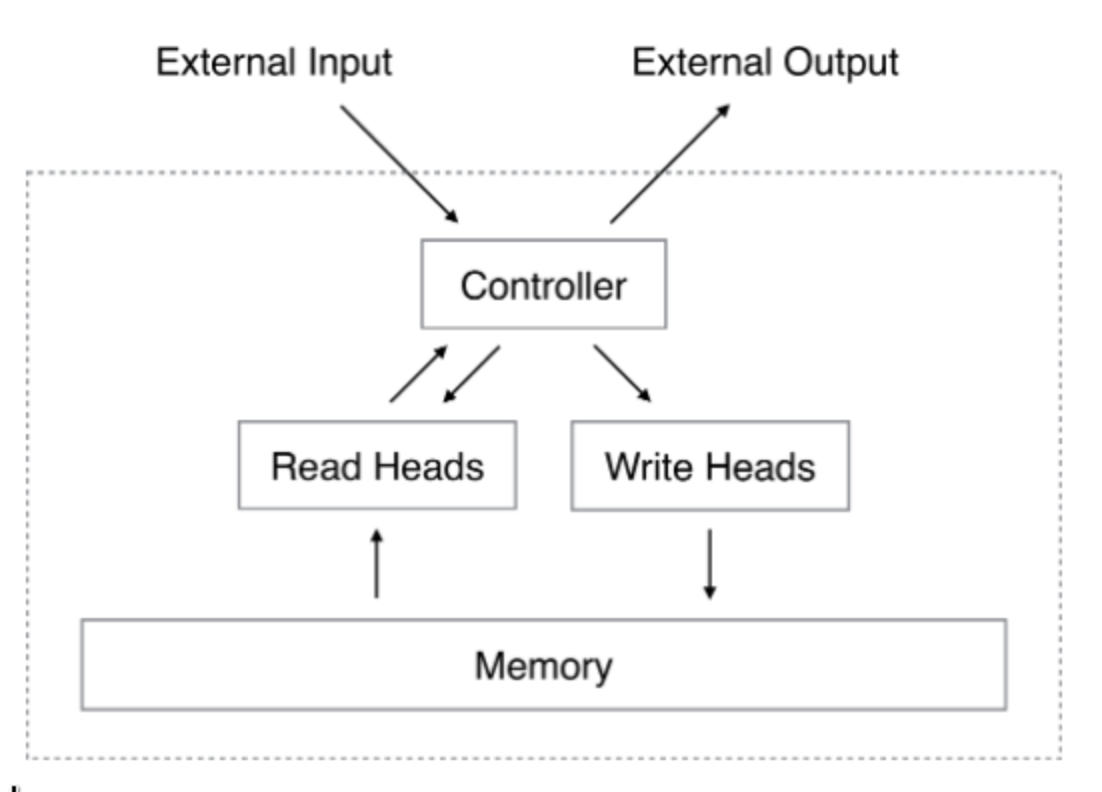
\includegraphics[width=7cm]{ntm}\vspace{-3mm}
	\\\small Neural Turing Machine Architecture \cite{ntm}
\end{center}

\vspace{1cm}
   
This task (project) will be done by the author of this proposal as the project course for CIS 700-Neural Program Learning course offered by Prof. Katz.


\bibliographystyle{IEEEtran}
\bibliography{references}

\end{document}
%%%%%%%%%%%%%%%%%%%% TeXStudio Magic Comments %%%%%%%%%%%%%%%%%%%%%
%% These comments that start with "!TeX" modify the way TeXStudio works
%% For details see http://texstudio.sourceforge.net/manual/current/usermanual_en.html   Section 4.10
%%
%% What encoding is the file in?
% !TeX encoding = UTF-8
%% What language should it be spellchecked?
% !TeX spellcheck = en_US
%% What program should I compile this document with?
% !TeX program = pdflatex
%% Which program should be used for generating the bibliography?
% !TeX TXS-program:bibliography = txs:///bibtex
%% This also sets the bibliography program for TeXShop and TeXWorks
% !BIB program = bibtex

%%% Local Variables:
%%% mode: latex
%%% TeX-master: t
%%% End:

